\section{Documentation LOGO et extensions}
\label{sec:Documentation}
\subsection{Modules de base}
\begin{table}[h!]
    \centering
    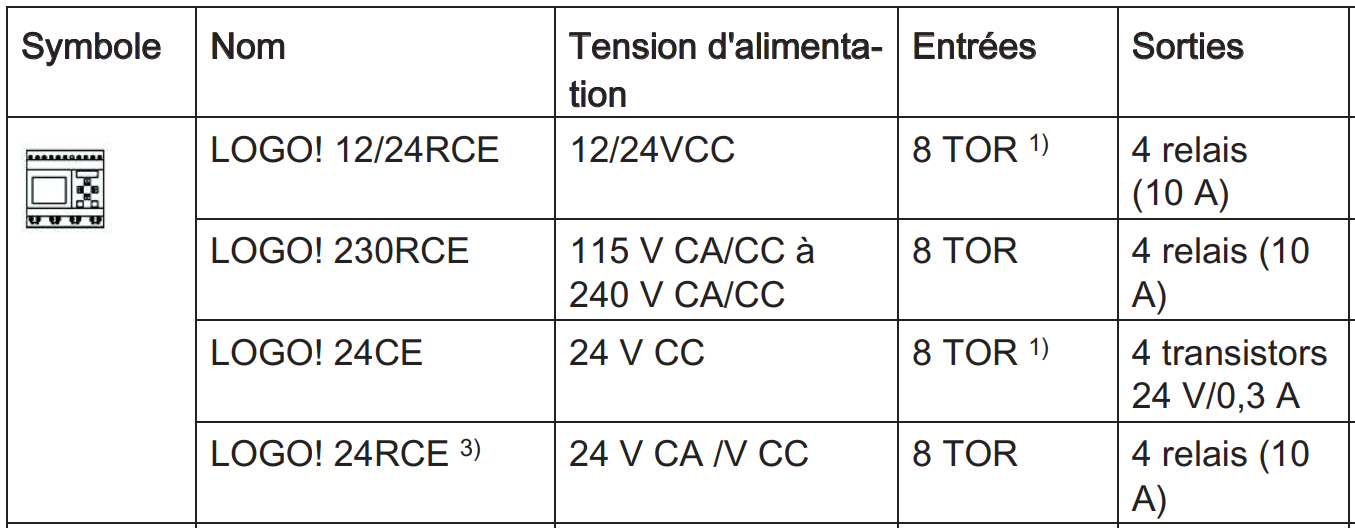
\includegraphics[width=\textwidth,height=.4\textheight,keepaspectratio]{images/doc_base_logo}
    \caption{Caractéristiques du module de base}
\end{table}

\subsection{Modules d'extension}
\begin{table}[h!]
    \centering
    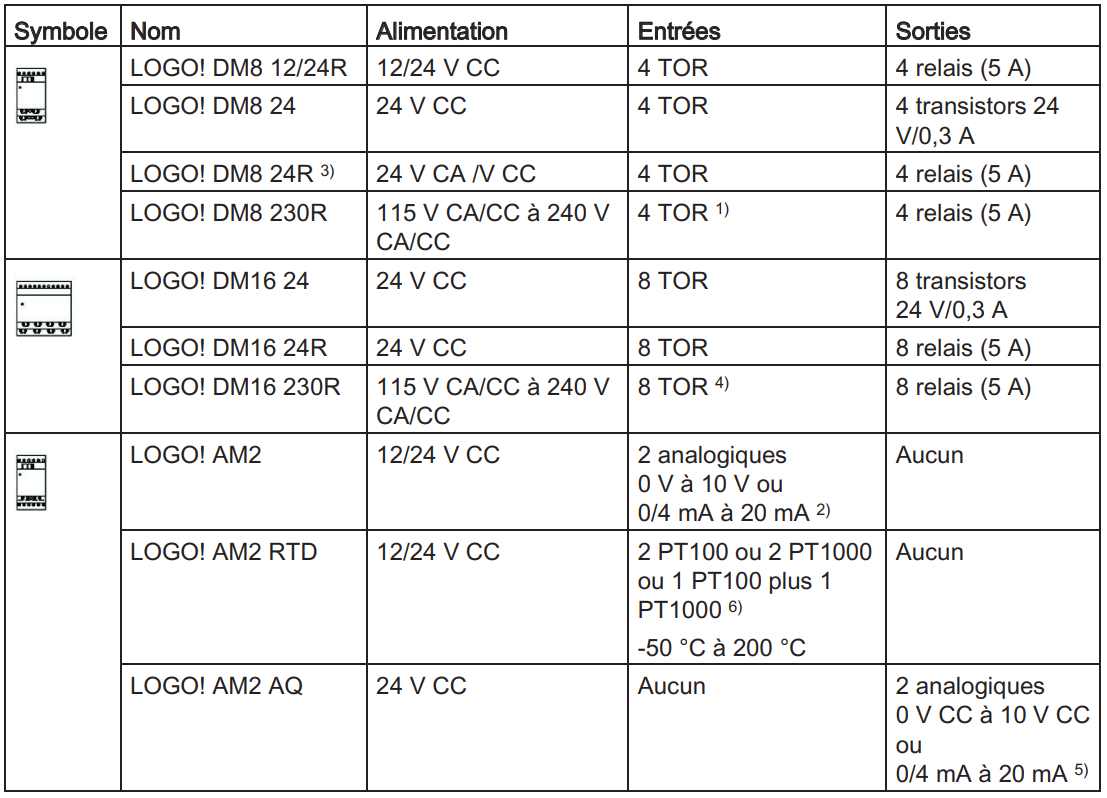
\includegraphics[width=\textwidth,height=.4\textheight,keepaspectratio]{images/doc_extension_logo.png}
    \caption{Caractéristiques du module de base}
\end{table}
\pagebreak
\subsection{Cablage de l'alimentation est des entrées}
\begin{figure}[h!]
    \centering
    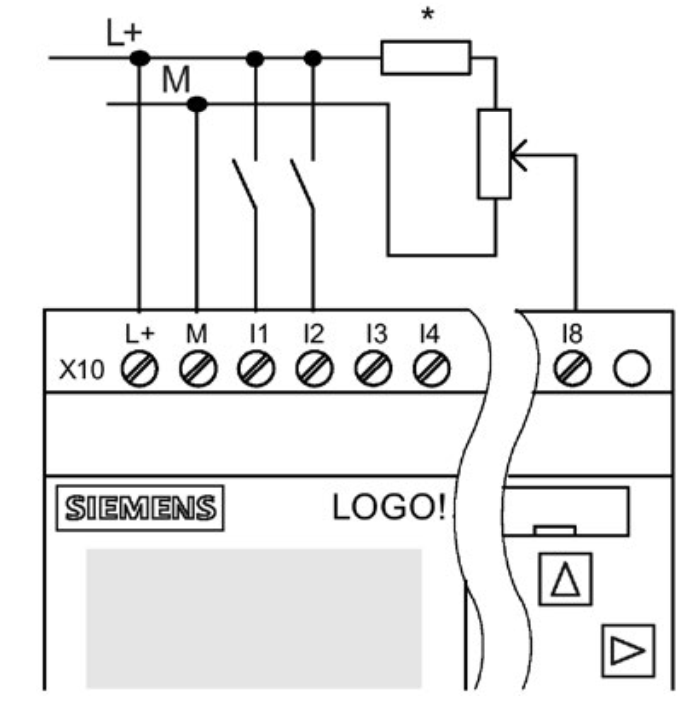
\includegraphics[width=\textwidth,height=.3\textheight,keepaspectratio]{images/cablage_alimentation_entrees.png}
    \caption{Cablage de l'alimentation et des entrées sur le module de base}
\end{figure}

\subsection{Cablage des sorties à relais}
\begin{figure}[h!]
    \centering
    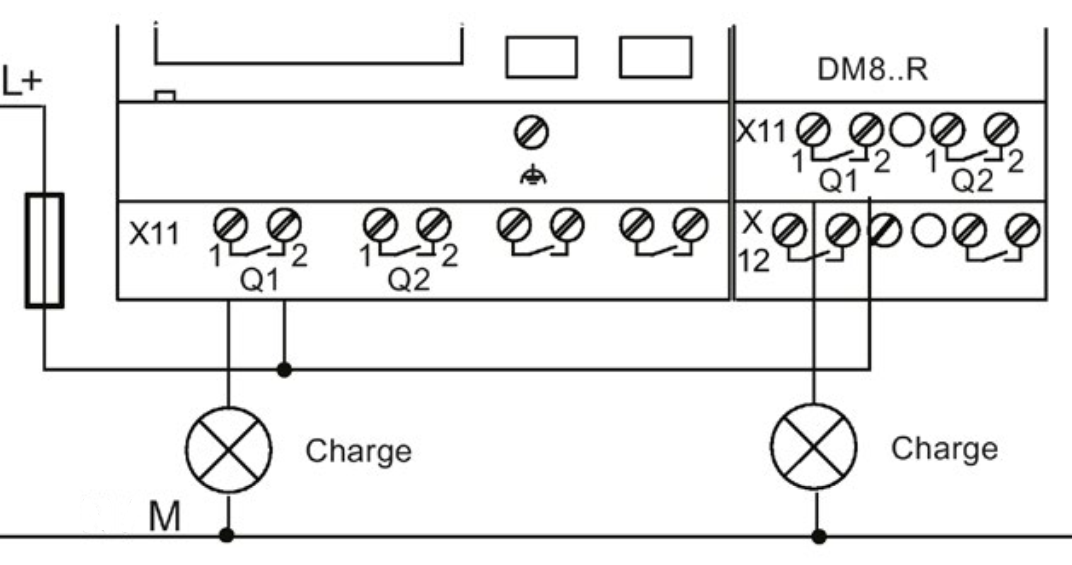
\includegraphics[width=\textwidth,height=.3\textheight,keepaspectratio]{images/cablage_sorties_relais.png}
    \caption{Cablage de l'alimentation et des entrées sur le module de base}
\end{figure}